% PRD flow chart 3: two ways of putting the SR source on the contour.
\documentclass[tikz,border=2pt]{standalone}
\usepackage[T1]{fontenc}
\usepackage{lmodern}
\usepackage{amsmath,amssymb}
\usetikzlibrary{arrows.meta,positioning,calc}
\newcommand{\PP}{\Phi^{\rm P}}
\newcommand{\Pres}{\Phi^{\rm res}}
\begin{document}
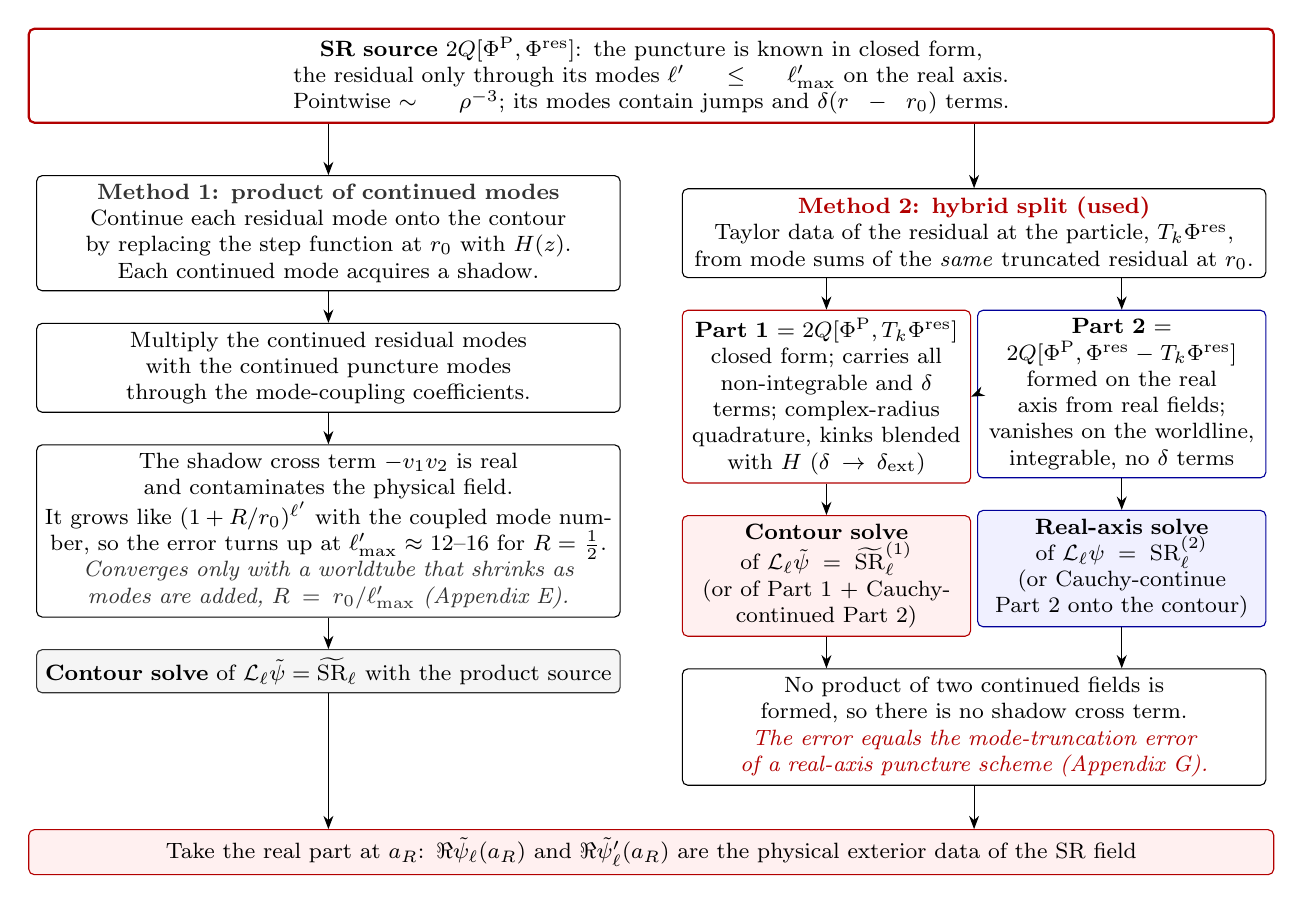
\begin{tikzpicture}[>=Stealth, font=\footnotesize,
  box/.style={draw, rounded corners=2pt, align=center, inner sep=3pt, text width=#1, fill=white},
  head/.style={font=\footnotesize\bfseries, align=center, text width=7.2cm}]
\node[box=15.6cm, draw=red!70!black, thick] (top) at (0,0)
  {\textbf{SR source} $2Q[\PP,\Pres]$: the puncture is known in closed form, the residual only through its modes $\ell'\le\ell'_{\max}$ on the real axis.\\
   Pointwise $\sim\rho^{-3}$; its modes contain jumps and $\delta(r-r_0)$ terms.};
% left column: product of continued modes
\node[box=7.2cm] (l1) at (-4.1,-2.0)
  {\textcolor{gray!40!black}{\textbf{Method 1: product of continued modes}}\\Continue each residual mode onto the contour by replacing the step function at $r_0$ with $H(z)$.\\
   Each continued mode acquires a shadow.};
\node[box=7.2cm] (l2) [below=0.40cm of l1]
  {Multiply the continued residual modes with the continued puncture modes through the mode-coupling coefficients.};
\node[box=7.2cm] (l3) [below=0.40cm of l2]
  {The shadow cross term $-v_1v_2$ is real and contaminates the physical field.\\
   It grows like $(1+R/r_0)^{\ell'}$ with the coupled mode number, so the error turns up at $\ell'_{\max}\approx12$--$16$ for $R=\tfrac12$.\\
   \textit{\textcolor{gray!40!black}{Converges only with a worldtube that shrinks as modes are added, $R=r_0/\ell'_{\max}$ (Appendix~E).}}};
% right column: hybrid split
\node[box=7.2cm] (r1) at (4.1,-2.0)
  {\textcolor{red!70!black}{\textbf{Method 2: hybrid split (used)}}\\Taylor data of the residual at the particle, $T_k\Pres$, from mode sums of the \emph{same} truncated residual at $r_0$.};
\node[box=3.45cm, draw=red!70!black] (r2a) [below=0.40cm of r1.south west, anchor=north west]
  {\textbf{Part 1} $=2Q[\PP,T_k\Pres]$\\closed form; carries all non-integrable and $\delta$ terms; complex-radius quadrature, kinks blended with $H$ ($\delta\to\delta_{\rm ext}$)};
\node[box=3.45cm, draw=blue!60!black] (r2b) [below=0.40cm of r1.south east, anchor=north east]
  {\textbf{Part 2} $=2Q[\PP,\Pres-T_k\Pres]$\\formed on the real axis from real fields; vanishes on the worldline, integrable, no $\delta$ terms};
\node[box=3.45cm, draw=red!70!black, fill=red!6] (r3a) [below=0.40cm of r2a]
  {\textbf{Contour solve} of $\mathcal L_\ell\tilde\psi=\widetilde{\mathrm{SR}}^{(1)}_\ell$\\(or of Part 1 $+$ Cauchy-continued Part 2)};
\node[box=3.45cm, draw=blue!60!black, fill=blue!6] (r3b) [below=0.40cm of r2b]
  {\textbf{Real-axis solve} of $\mathcal L_\ell\psi=\mathrm{SR}^{(2)}_\ell$\\(or Cauchy-continue Part 2 onto the contour)};
\node[box=7.2cm] (r4) [below=0.40cm of r3a.south west, anchor=north west]
  {No product of two continued fields is formed, so there is no shadow cross term.\\
   \textit{\textcolor{red!70!black}{The error equals the mode-truncation error of a real-axis puncture scheme (Appendix~G).}}};
\node[box=7.2cm, draw=gray!40!black, fill=gray!8] (lbot) [below=0.40cm of l3]
  {\textbf{Contour solve} of $\mathcal L_\ell\tilde\psi=\widetilde{\mathrm{SR}}_\ell$ with the product source};
\path let \p1=(lbot.south), \p2=(r4.south) in coordinate (lowest) at (0,{min(\y1,\y2)});
\node[box=15.6cm, draw=red!70!black, fill=red!6] (bot) [below=0.55cm of lowest]
  {Take the real part at $a_R$: $\Re\tilde\psi_\ell(a_R)$ and $\Re\tilde\psi'_\ell(a_R)$ are the physical exterior data of the SR field};
\draw[->] (top.south -| l1) -- (l1.north);
\draw[->] (top.south -| r1) -- (r1.north);
\draw[->] (l1) -- (l2); \draw[->] (l2) -- (l3);
\draw[->] (r1.south -| r2a) -- (r2a.north);
\draw[->] (r1.south -| r2b) -- (r2b.north);
\draw[->] (r2a.south) -- (r3a.north);
\draw[->] (r2b.south) -- (r3b.north);
\draw[->, dashed] (r2b.west) -- (r2a.east);
\draw[->] (r3a.south) -- (r3a.south |- r4.north);
\draw[->] (r3b.south) -- (r3b.south |- r4.north);
\draw[->] (l3.south) -- (lbot.north);
\draw[->] (lbot.south) -- (lbot.south |- bot.north);
\draw[->] (r4.south) -- (r4.south |- bot.north);
\end{tikzpicture}
\end{document}
